\documentclass{beamer}
\usepackage{tikz}
\usetikzlibrary{shapes, arrows}
\usetheme{metropolis}

% define block styles
\tikzstyle{rounded} = [rectangle, draw, text centered, rounded corners]
\tikzstyle{parallo} = [trapezium,trapezium left angle=70,trapezium right angle=-70, draw, text centered]
\tikzstyle{box} = [rectangle, draw, text centered]
\tikzstyle{line} = [draw, -latex]

\title{Automatic Speech Recognition System}
\subtitle{OOAD Project}
\author{
  Bikash Gupta(070BCT-512)\\
  Kshitiz Shrestha(070BCT-518)\\
  Miran Ghimire(070BCT-521)\\
  Nabin Bhattarai(070BCT-522)\\
  Pabin Raj Luitel(070BCT-523)\\
  Sabin Silwal(070BCT-532)
}
\institute{IOE, Central Campus Pulchowk}
\date{\today}


\begin{document}
\begin{frame}
\titlepage
\end{frame}

\begin{frame}
  \centering
  \frametitle{History Of Speech Recognition}
  \begin{itemize}
  \item 1930s: Bell Lab's investigation in speech perception.
    \pause
  \item 1950s: Single-Speaker digit recognition system.
    \pause
  \item 1960s: Rise of Hidden Markov Model.
    \pause
  \item 1970s: Development of DARPA(Defense Advanced Research Projects Agency) SR.
    \pause
  \item 1980s: Limited vocabulary based speech recognition system.
    \pause
  \item 1990s: First commercially successful speech recognition technologies.
    \pause
  \item $21^{st}$ Century : Effective systems with deep learning and LSTM(Long short-term memory).
  \end{itemize}
\end{frame}

\begin{frame}
  \centering
  \frametitle{Speech Recognition}
  \begin{itemize}
    \pause
  \item Translating spoken words into text.
    \pause
  \item It is very Hard due to
    \pause
    \begin{itemize}
    \item Different Accent, Pronunciations, Styles, Rate of Speaker
      \pause
    \item Noise, different types of microphones.
    \end{itemize}
  \end{itemize}
\end{frame}

\begin{frame}
  \centering
  \frametitle{Usage Of ASR}
  \begin{itemize}
  \item Can be integrated with other digital system to make ease to use
    \pause
  \item Home Automation
    \pause
  \item Hands-free computing
    \pause
  \item Interactive voice response
    \pause
  \item Robotics
    \pause
  \item And Many more...
  \end{itemize}
\end{frame}

\begin{frame}[c]
  \frametitle{Project Overview}
  \centering
  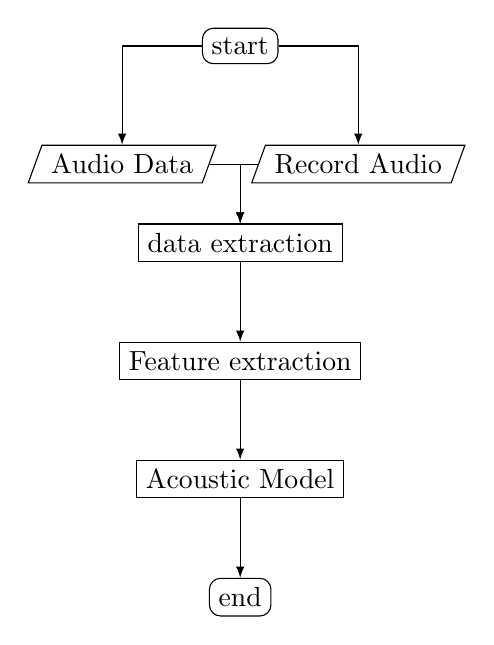
\begin{tikzpicture}[align=center, node distance=1.5cm]
    \node [rounded] (start) {start};
    \node [parallo, right of=start, below of=start] (record_audio) {Record Audio};
    \node [parallo, left of=start, below of=start] (audio_data) {Audio Data};
    \node [box, below of=start, node distance=2.5cm, align=center] (data_ext) {data extraction};
    \node [box, below of=data_ext] (feature_ext) {Feature extraction};
    \node [box, below of=feature_ext] (acoustic_model) {Acoustic Model};
    \node [rounded, below of=acoustic_model] (end) {end};

    \path [line] (start) -| (record_audio);
    \path [line] (start) -| (audio_data);
    \path [line] (record_audio) -| (data_ext);
    \path [line] (audio_data) -| (data_ext);
    \path [line] (data_ext) -- (feature_ext);
    \path [line] (feature_ext) -- (acoustic_model);
    \path [line] (acoustic_model) -- (end);
  
  \end{tikzpicture}
  \pause
  \cleardoublepage
  \textbf{haha}
\end{frame}

\begin{frame}
  
\end{frame}

\end{document}

%%% Local Variables:
%%% mode: latex
%%% TeX-master: t
%%% End:
